\section{Background}


% motivation

Hash tables are one of the most widely used data
structures in sequential programs. Data is stored by mapping a key to
a value. Values may be retrieved in a random access manner by
providing the key to get or put operations on the hash table.

% serial vs. parallel approaches
Hash tables can be implemented with a myriad of different techniques,
but are traditionally implemented sequentially as an array of pointers
to objects. Parallel implementations typically distribute table data
across nodes, requiring that the hash table stores the entire object
and not simply a reference.

% sparsity
\subsection{Sparsity}
Of interest to the HPC community, we see parallel hash tables as a
means for dealing with sparsity. Many common HPC applications rely on
sparse data structures, which causes numerous problems in the hunt for
high performance. Matrix and tensor representations often must contend
with sparse data, resulting in specialized formats such compressed
sparse row (CSR) and variants. Other problems, such as N-body
simulation, grid and mesh solvers, are naturally expressed using
spatial decomposition trees such as quadtrees and octrees. 

In these cases, there is a natural mapping between an index or
coordinate system and the corresponding data. A global distributed
hash table could replace a complicated and difficult to parallelize
sparse data structures given the right application.

\subsection{Related Work}

Other people have done things like this before.

\section{Portals 4}

% portals background

% figure 2.2 / 2.3 in portals spec

%  define NI, PTE
%     - target vs. initiator
%     - wrt SPMD each process plays both roles
%     - define memory descriptor
%     - like a window w MPI?

%  matching interface
%      - define matching, 
%      - ME 
%      -  matching lookup process
%      - priority list

%  define counters and events
%       - define event and counter abstractions
%       - target vs. initiator events / counters
%       - attached to either MD, ME, or PTE
%       - define ct
%            - success vs. failure events
%       - define event
%            - put - target gets put data in event
%            - ack - operation complete
%            - reply - operation completed
%            - flow control


% use figure* to span both cols
\begin{figure}[ht]
  \centering
  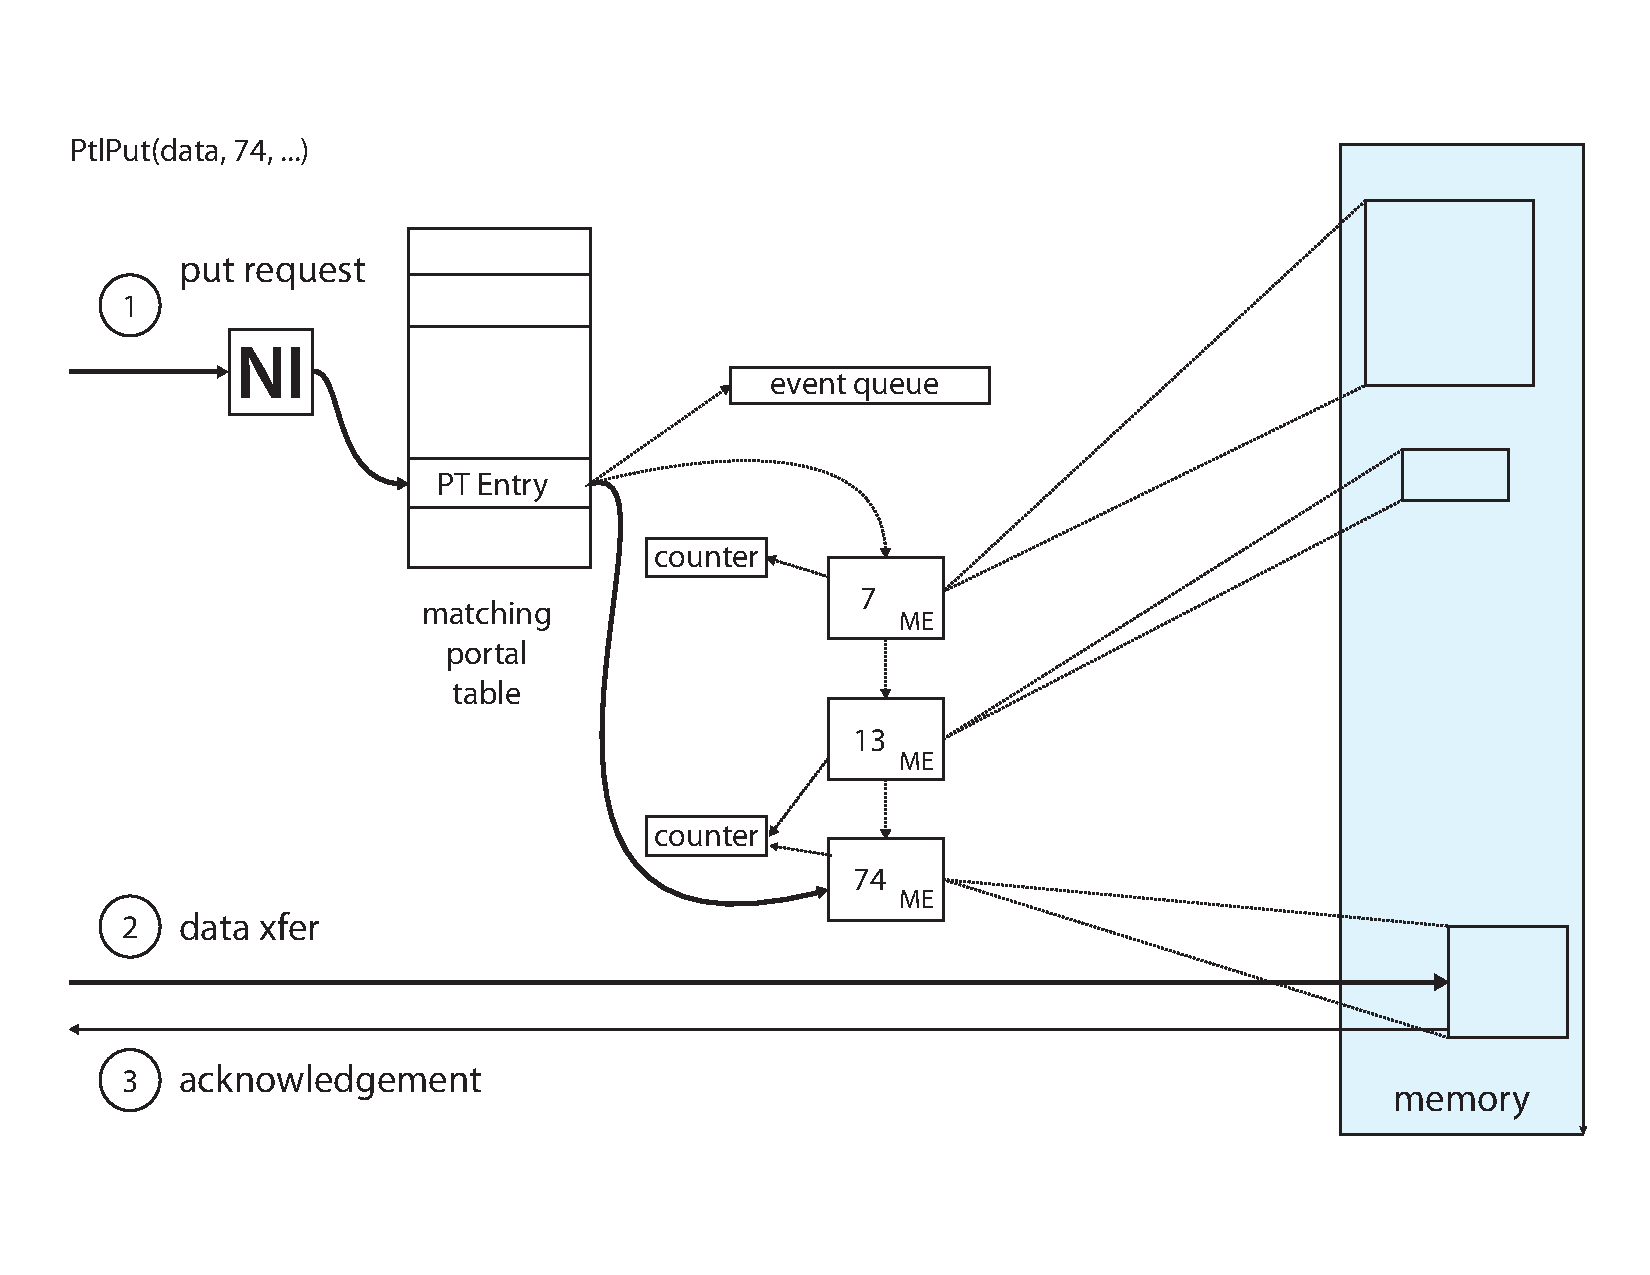
\includegraphics[scale=.35]{figs/portals_put}
  \caption{Portals data structures and example put operation.}
  \label{fig:portals_put}
\end{figure}


The Portals framework uses several low-level data abstractions that
are used to implement the \pdht system. \pdht is based on a one-sided
communication model to avoid the need for matched/blocking calls and
additional synchronization. While Portals provides support for both
one-sided and matched message-passing semantics, a novel feature of
this project is to utilize the Portals' matching interface
abstractions to implement a one-sided model that is the basis for
\pdht. By using features in the Portals library in a unique fashion,
we can take advantage of network hardware offload  to a greater extent
than conventional PGAS techniques. Portals defines several concepts
and abstractions that are necessary to the understanding of the
\pdht. The relationship between these different entities is shown in
Figure \ref{fig:portals_put}.

Portals defines two primary roles for communication operations. The
{\em initiator} is the process that is issuing the communication
request and the {\em target} is the process receiving the
requests. The initator defines a {\em memory descriptor} (MD), a
region to be used for Portals operations and is able to check the
success or failure of various events. Specific completion information
and notifications may be only visible to the initiator and not the
target, or vice versa.

Portals specifies a {\em network interface} (NI) as a per-process
abstraction of a physical network interface on the target process.The
NI is defined at creation to be either a {\em matching} or a {\em
  non-matching} interface, depending on the intended use for the
interface (message-passing or one-sided). \pdht relies on the Portals
matching interface.

Each NI is associated with a portal table (PT). The index into the
portal table is specified on every Portals communication operation and
is used to separate and classify different channels between endpoints.
Every portal table entry (PTE) maintains a list of memory regions that
are available for communication operations as well as an event queue
to track asynchronous notifications for ongoing communication.

A PTE using the matching interface maintains a list of match-list
entries (ME). Each ME specifies a set of matching criteria and a
memory region associated with the entry. If all of the match criteria
are satisfied, the communication operation commences working on
corresponding memory region. In particular, each ME contains a 64-bit
{\em match bits} field that must match exactly for an incoming
communication to proceed with the given ME. For example, a process
would post an {\tt MPI\_Recv()} with a specific match bits
field. Later, Portals would receive a communication request for an
{\tt MPI\_Send()} with the same match bits, which would be correspond
to the posted receive.

Additionally, Portals provides both {\em event queues} and {\em event
  counters} to track the data movement in and out of memory regions
used by Portals operations. Both events and counters are also used to
log failure events and other information. 

Events are detailed descriptions of communcation activities. They may
contain pointers to the transmitted data, send/receive parameters,
etc. An event queue may be associated with either the initiator
process or the target process.  On the initiator, an event queue may
be associated with the memory descriptor (MD), whereas on the target,
an event queue may be associated with each PTE. 

Counters are useful for lightweight event counting, where copying a
large amount of data from the Portals implementation to the
application is unneccessary. Counters track the count of both
successful and failed communicadtion operations and are designed to
support efficient one-sided communication models. Like event queues, a
counter may be associated with either initiator or target
processes. Unlike target-side event queues, a counter may be
associated with each ME in the match-list. Multiple MEs may share a
single counter, if desired. \pdht typically uses counters to watch for
successful completion, and events to track specific failures. More
detailed descriptions of event and counter use within \pdht is
discussed below.

To put everything together, Figure \ref{fig:portals_put} shows the
relationships between the target-side data structures and a sample
{\tt PtlPut()} operation. In this example, we assume that the
initiator process has called {\tt PtlPut} with some data on a matching
interface, with the expected match bits set to 74. When the target
process receives the request, it is dispatched through the
initiator-specified PT index. Next, the match list is searched, until
a 74 is found, or the end of the list is reached. Once the ME has been
located, the PtlPut data is copied into the corresponding memory
region. The operation may cause a {\tt PUT} event to be appended to
the event queue or ME success counter to be incremented. An
acknowledgement is sent back to the initiator, possibly generating
another full event or counting event.



%reply: initiator: remote completion of a get: success = got it, failure = not
%found
%ack: initiator:  put completed
%put: target -> event with put data / ME
%flow control: initiator: disabled NI 

%%% Local Variables:
%%% mode: latex
%%% TeX-master: "paper"
%%% End:
